\documentclass[xcolor=table]{beamer}
\usepackage{beamerthemesplit}
\usepackage{wrapfig}
\usetheme{SPbGU}
\usepackage{pdfpages}
\usepackage{amsmath}
\usepackage{amssymb}
\usepackage{cmap}
\usepackage[T2A]{fontenc}
\usepackage[utf8]{inputenc}
\usepackage[english]{babel}
\usepackage{indentfirst}
\usepackage{tikz}
\usetikzlibrary{shapes,arrows,automata,positioning,quotes,backgrounds,decorations.text,decorations.pathmorphing}
\usepackage{multirow}
\usepackage[noend]{algpseudocode}
\usepackage{algorithm}
\usepackage{algorithmicx}
\usepackage{fancyvrb}
\usepackage[linguistics]{forest}
\usepackage{listings}
\usepackage{multicol}
\usepackage{comment}
\usepackage{xspace}
\usepackage{adjustbox}
\usepackage{makecell}
\usepackage{proof}

\setbeamertemplate{itemize items}[circle]
\setbeamertemplate{enumerate items}[circle]

\lstdefinelanguage{ocanren}{
keywords={run, conde, fresh, let, in, match, with, when, class, type,
object, method, of, rec, repeat, until, while, \begin{comment}not,\end{comment} do, done, as, val, inherit,
new, module, sig, deriving, datatype, struct, if, then, else, open, private, virtual, include, success, failure,
true, false},
sensitive=true,
commentstyle=\small\itshape\ttfamily,
keywordstyle=\textbf,%\ttfamily\underline,
identifierstyle=\ttfamily,
basewidth={0.5em,0.5em},
columns=fixed,
mathescape=true,
fontadjust=true,
literate={fun}{{$\lambda$}}1 {function}{function}8 {->}{{$\to$}}3 {===}{{$\equiv$}}1 {=/=}{{$\not\equiv$}}1 {|>}{{$\triangleright$}}3 {\\/}{{$\vee$}}2 {/\\}{{$\wedge$}}2 {^}{{$\uparrow$}}1,
morecomment=[s]{(*}{*)},
 moredelim=**[is][\color{red}]{@!}{@}
}

\tikzstyle{processTree} = [
  ->,
  sibling distance=15em,
  scale=0.6,
  every node/.style = {
    shape=rectangle,
    rounded corners=0.05cm,
    draw,
    align=center,
    minimum size=5mm,
    scale=0.6,},
  %level 1/.style={sibling distance=100em}
  ]


\tikzstyle{program} = [
  draw=black,
  thick,
  rectangle,
  rounded corners=1pt,
  inner sep=5pt,
  inner ysep=5pt
  ]

\tikzstyle{goal} = [
  draw=black,
  rectangle,
  rounded corners=1pt,
  inner ysep=0pt,
  ]

\tikzstyle{input} = [
  draw=none,
  rectangle,
  rounded corners=1pt,
  inner sep=2pt,
  inner ysep=2pt,
  fill=green!10,
  minimum height=5mm
  ]


\tikzstyle{transparent} = [
  draw=none,
  inner ysep=3pt
  ]

\lstset{
language=ocanren
}

\newcommand{\mk}{\textsc{miniKanren}\xspace}
\renewcommand{\and}{$\&$\xspace}
\newcommand{\rel}[2]{\texttt{#1}$^o$ #2}
\newcommand{\subst}[1]{$\langle$#1$\rangle$}

\beamertemplatenavigationsymbolsempty

\title[Partial Deduction for \mk{}]{An Empirical Study of Partial Deduction for \mk{}}
\institute[JetBrains Research]{
JetBrains Research, Programming Languages and Tools Lab  \\
Saint Petersburg State University
}

\author[Kate Verbitskaia]{\textbf{Kate Verbitskaia}, Daniil Berezun, Dmitry Boulytchev}

\date{28.03.2021}

\definecolor{orange}{RGB}{179,36,31}

\begin{document}
{
\begin{frame}[fragile]
  \begin{tabular}{p{5.5cm} p{5.5cm}}
   \begin{center}
      
\includegraphics[height=1.5cm]{pictures/jetbrainsResearch.pdf}
    \end{center}
    &
    \begin{center}
      
\includegraphics[height=1.5cm]{pictures/SPbGU_Logo.png}
    \end{center}
  \end{tabular}
  \titlepage
\end{frame}
}

\begin{frame}[fragile]
  \frametitle{\mk: Relational Programming Language (Family)}
  \begin{center}
      \begin{tikzpicture}[
  scale=0.8,
  every node/.style = {
    shape=rectangle,
    rounded corners=0.05cm,
    draw,
    align=center,
    minimum size=5mm,
    scale=0.8,},
  node distance=1.3em,
  anchor=center
]
  \node[inner sep=10pt] (code) at (0,0) {\begin{lstlisting}
let rec append$^o$ x y r =
  ocanren {
    (x === [] & y === r) |
    (fresh h x' r' in
      x === h :: x' &
      append$^o$ x' y r' &
      r === h :: r')}
    \end{lstlisting}};
    \node (em) [draw=none, left=of code, yshift=3cm] {embedded};
    \node (rel) [draw=none, right=of code, yshift=3cm] {relation};
    \draw [red,<-] ($(code.west)+(0.6,0.9)$) to [out=180,in=-90] node[below, draw=none, red] {} ($(em.south)+(0,0)$);
    \draw [red,<-] ($(code.north)+(0,-0.4)$) to [out=90,in=180] node[below, draw=none, red] {} ($(rel.west)+(0,0)$);

    \pause

    \node (disj) [draw=none, right=of code, yshift=0.4cm] {disjunction};
    \node (conj) [draw=none, right=of code, yshift=-1cm] {conjunction};
    \node (uni) [draw=none, left=of code, yshift=0.4cm] {term unification};
    \node (fresh) [draw=none, left=of code, yshift=-1cm] {variable introduction};
    \node (call) [draw=none, below=of code] {relation call};

    \draw [red,<-] ($(code.south)+(-1.2,1.1)$) to [out=-180,in=135] node[below, draw=none, red] {} ($(call.north west)+(0,0)$);

    \draw [red,<-] ($(code.west)+(1.6,0.55)$) to [out=150,in=0] node[below, draw=none, red] {} ($(uni.east)+(0,0)$);

    \draw [red,<-] ($(code.west)+(1.4,-0.3)$) to [out=230,in=0] node[below, draw=none, red] {} ($(fresh.east)+(0,0)$);


    \draw [red,<-] ($(code.east)+(-0.6,0.4)$) to [out=0,in=-180] node[below, draw=none, red] {} ($(disj.west)+(0,0)$);

    \draw [red,<-] ($(code.east)+(-0.3,-1)$) to [out=0,in=-180] node[below, draw=none, red] {} ($(conj.west)+(0,0)$);
    \draw [red,<-] ($(code.east)+(-1.1,-0.5)$) to [out=0,in=-190] node[below, draw=none, red] {} ($(conj.west)+(0,0)$);

  \end{tikzpicture}
  \end{center}
\end{frame}

\begin{frame}[fragile]
  \frametitle{\mk: Querying}
  \begin{columns}
    \begin{column}{0.4\textwidth}
      \begin{center}
        \begin{lstlisting}
let rec append$^o$ x y r =
  ocanren {
    (x === [] & y === r) |
    (fresh h x' r' in
      x === h :: x' &
      append$^o$ x' y r' &
      r === h :: r')}
\end{lstlisting}
      \end{center}
    \end{column}
    \begin{column}{0.6\textwidth}
      \begin{itemize}
        \item \lstinline{fresh q in append$^o$ [1] [2] q}
        \begin{itemize}
          \setlength{\itemindent}{-0.6em}
          \item \lstinline{$\langle$ q $\to$ [1,2] $\rangle$}
        \end{itemize}
        \item \lstinline{fresh x, y in append$^o$ x y [1,2]}
        \begin{itemize}
          \setlength{\itemindent}{-0.6em}
          \item \lstinline{$\langle$ x $\to$ [], y $\to$ [1,2] $\rangle$}
          \item \lstinline{$\langle$ x $\to$ [1], y $\to$ [2] $\rangle$}
          \item \lstinline{$\langle$ x $\to$ [1,2], y $\to$ [] $\rangle$}
        \end{itemize}
        \item \lstinline{fresh x, y, z in append$^o$ x y z}
        \begin{itemize}
          \setlength{\itemindent}{-0.6em}
          \item \lstinline{$\langle$ x $\to$ [], y $\to$ $\__0$, z $\to$ $\__0$ $\rangle$}
          \item \lstinline{$\langle$ x $\to$ $[\__0]$, y $\to$ $\__1$, z $\to$ $(\__0 : \__1)$ $\rangle$}
          \item $\dots$
        \end{itemize}
      \end{itemize}
    \end{column}
  \end{columns}

\end{frame}

\begin{frame}[fragile]
  \frametitle{Relational Interpreters for Search Problems}
  \begin{center}
    Recognizer backwards = solver
  \end{center}

  \begin{itemize}
    \item Write recognizer in functional language
    \item Run relational conversion to get relational interpreter from the recognizer
    \item Run relational interpreter backwards
  \end{itemize}

\begin{center}
  Core issue: running relational interpreter backwards is slow
\end{center}

\begin{center}
  Possible solution: partial deduction
\end{center}
\end{frame}


\begin{frame}[fragile]
  \frametitle{Partial Deduction: a Method to Improve Logic Programs}
\begin{center}
  \begin{tikzpicture}[
  node distance = 10mm and 11 mm,
  decoration = {
    snake,
    pre length=2pt,
    post length=2pt
  },
  remember picture,
  overlay]
  \node (a) [
    program,
    anchor=north west,
    xshift=0.4cm,
    yshift=-1.7cm]
  at (current page.north west)
  {
    \adjustbox{scale=0.7}{
      \begin{minipage}[c]{0.63\textwidth}
        \begin{lstlisting}
let rec eval$^o$ fm s r =
  fm === neg x & not$^o$ a r & eval$^o$ x s a |
  ...
        \end{lstlisting}
      \end{minipage}
    }
  };

  \node [transparent,anchor=south] at (a.north) {
    \footnotesize
    input program
  };

  \pause

  \node (c) [goal,anchor=north east] at (a.south east)
  {
    \adjustbox{scale=0.7}{
      \begin{minipage}[c]{0.25\textwidth}
        \begin{lstlisting}
eval$^o$ fm s true
        \end{lstlisting}
      \end{minipage}
    }
  };

  \node (lbl) [transparent,anchor=south west] at (a.east) {
    \footnotesize
    known argument
  };

  \draw [dashed,->] (lbl.south) to [out=270,in=0] ($(c.east)-(0.2,0)$);
  \pause

  \node (d) [input, below=of a]
  {
    \adjustbox{scale=0.7}{
      \begin{minipage}[c]{0.65\textwidth}
        \begin{lstlisting}
fm === neg x & not$^o$ a true & eval$^o$ x s a |
...
        \end{lstlisting}
      \end{minipage}
    }
  };

  \path[draw=black,->,thick, decorate] (a.south) to (d.north);

  \pause

  \node (e) [input, below=of d]
  {
    \adjustbox{scale=0.7}{
      \begin{minipage}[c]{0.5\textwidth}
        \begin{lstlisting}
fm === neg x & eval$^o$ x s false |
...
        \end{lstlisting}
      \end{minipage}
    }
  };

  \path[draw=black,->,thick, decorate] (d.south) to (e.north);

  \pause

  \node (dots) [input, below=of e] {...};

  \path[draw=black,->,thick, decorate] (e.south) to (dots.north);

  \pause

  \node (b) [
    program,
    anchor=south east,
    xshift=-0.4cm,
    yshift=0.7cm]
  at (current page.south east)
  {
    \adjustbox{scale=0.7}{
      \begin{minipage}[c]{0.53\textwidth}
        \begin{lstlisting}
let rec eval_true$^o$ fm s =
  fm === neg x & eval_false$^o$ x s |
  ...

let rec eval_false$^o$ fm s =
  fm === neg x & eval_true$^o$ x s |
  ...
        \end{lstlisting}
      \end{minipage}
    }
  };

  \node [transparent,anchor=south] at (b.north) {
    \footnotesize
    output
  };
\onslide<1->
\end{tikzpicture}

\end{center}
\end{frame}

\begin{frame}[fragile]
  \frametitle{Partial Deduction for \mk: Bird's-eye View}
  \begin{center}
\begin{tikzpicture}[
  node distance = 14mm and 13 mm,
  decoration = {
    snake,
    pre length=2pt,
    post length=4pt,
    amplitude=0.5pt,
    segment length=4pt
  },
  remember picture,overlay]
  \node (a) [
    program,
    anchor=north west,
    xshift=1cm,
    yshift=-1.8cm]
  at (current page.north west)
  {
    \adjustbox{scale=0.65}{
      \begin{minipage}[c]{0.38\textwidth}
        \begin{lstlisting}
let rec eval$^o$ fm s r =
  ...
  fm === conj x y &
  and$^o$ a b r &
  eval$^o$ x s a &
  eval$^o$ y s b |
  ...
        \end{lstlisting}
      \end{minipage}
    }
  };

  \node (b) [goal,anchor=north east] at (a.south east)
  {
    \adjustbox{scale=0.65}{
      \begin{minipage}[c]{0.24\textwidth}
        \begin{lstlisting}
eval$^o$ fm s true
        \end{lstlisting}
      \end{minipage}
    }
  };

  \pause

  \node (d) [
    transparent,
    xshift=-1cm,
    yshift=-1.8cm,
    anchor=north east]
  at (current page.north east)
  {
      \begin{tikzpicture}[
  processTree,
  sibling distance=7em,
  level distance=7em,
  level 2/.style={level distance=5em},
  anchor=center]
  \node {
    \rel{eval}{$fm \ s \ true$}}
    child { node[draw=none, fill=none] {...}}
    child { node {
      \rel{and}{$a \ b \ true$} \and  \\
      \rel{eval}{$x \ s \ a$} \and \\
      \rel{eval}{$y \ s \ b$} \\
      \subst{$fm \to conj \ x \ y$}}
      child { node[draw=none, fill=none] {...}}
      }
    child { node[draw=none, fill=none] {...}}
  ;
\end{tikzpicture}
  };

  \draw[->,semithick, decorate]
    (a.north east) to
    [out=15,in=165,"{\footnotesize driving}"]
    ($(d.north west)+(0.9,0)$);

  \pause

  \node (e) [transparent, anchor=north east] at ($(d.south east)+(0,-1)$)
  {
    \begin{minipage}[c]{0.4\textwidth}
      \begin{tikzpicture}[
  processTree,
  sibling distance=4em,
  level distance=3em,
  level 3/.style={level distance=4em,sibling distance=8em},
  anchor=center]
  \node (root) {
    \rel{eval}{$fm \ s \ true$}}
    child { node[draw=none, fill=none] {...}}
    child { node[draw=none, fill=none] {...}
      child { node {
        \rel{eval}{$x \ s \ true$} \and \\
        \rel{eval}{$y \ s \ true$}}
        child { node (1) {\rel{eval}{$x \ s \ true$}}}
        child { node (2) {\rel{eval}{$y \ s \ true$}}}
        }
    }
    child { node[draw=none, fill=none] {...}}
  ;

  \draw [dashed,->] (1.west) to [out=170,in=-150] (root.west);
  \draw [dashed,->] (2.east) to [out=10,in=-30] (root.east);


\end{tikzpicture}
    \end{minipage}
  };

  \draw[->,semithick, decorate]
    ($(d.south)+(0.6,0.7)$) to
    [out=-75,in=45,"{\footnotesize folding}"]
    (e.north);

  \pause


  \node (c) [
    program,
    anchor=south west,
    xshift=1cm,
    yshift=0.8cm]
  at (current page.south west)
  {
    \adjustbox{scale=0.65}{
      \begin{minipage}[c]{0.4\textwidth}
        \begin{lstlisting}
let rec eval$^o$_true fm s =
  ...
  fm === conj x y &
  eval$^o$_true x s &
  eval$^o$_true y s |
  ...
        \end{lstlisting}
      \end{minipage}
    }
  };

  \draw[->,semithick, decorate]
    ($(e.west)+(0.45,0)$) to
    [out=200,in=-35,"{\footnotesize residualization}",pos=0.4]
    (c.east);

    \onslide<1->
\end{tikzpicture}
  \end{center}
\end{frame}

\begin{frame}[fragile]
  \frametitle{Driving: Unfolding}
  \begin{center}
    

\begin{tikzpicture}[
  decoration = {
    snake,
    pre length=2pt,
    post length=4pt,
    amplitude=0.5pt,
    segment length=4pt,
  },
  remember picture,overlay]
  % \draw[thick] (current page.south west) rectangle (current page.north east);
  \node (a) [
    program,
    anchor=north west,
    xshift=0.4cm,
    yshift=-1.4cm]
    at (current page.north west)
  {
    \adjustbox{scale=0.5}{
      \begin{minipage}[c]{0.68\textwidth}
        \begin{lstlisting}
let rec eval$^o$ fm s r =
  ...
  fm === conj x y & and$^o$ a b r &
  eval$^o$ x s a & eval$^o$ y s b |
  ...
        \end{lstlisting}
        \begin{lstlisting}
let and$^o$ x y r =
  ocanren {
    fresh xy in
      (nand$^o$ x y xy & nand$^o$ xy xy r) }

let rec nand$^o$ x y r =
  ocanren {
    (x === true & y === true & r === false) |
    (x === true & y === false & r === true) |
    (x === false & y === true & r === true) |
    (x === false & y === false & r === true) }
\end{lstlisting}
      \end{minipage}
    }
  };

  \node (b) [goal,anchor=north east] at (a.south east)
  {
    \adjustbox{scale=0.5}{
      \begin{minipage}[c]{0.24\textwidth}
        \begin{lstlisting}
eval$^o$ fm s true
        \end{lstlisting}
      \end{minipage}
    }
  };

  \pause

  \node (d) [
    transparent,
    anchor=north east,
    xshift=-0.4cm,
    yshift=-1.4cm]
    at (current page.north east)
  {
    \begin{tikzpicture}[
  processTree,
  anchor=center]
  \node (root) {\rel{eval}{$fm \ s \ true$}}
    child { node {$fm \equiv conj \ x \ y $ \and \rel{and}{$a \ b \ true$} \and \rel{eval}{$x \ s \ a$} \and \rel{eval}{$y \ s \ b$}}
      child { node {
        \rel{and}{$a \ b \ true$} \and
        \rel{eval}{$x \ s \ a$} \and
        \rel{eval}{$y \ s \ b$} \\
        \subst{$fm \to conj \ x \ y$}}
    }
    }
    ;

  \node[left=4em of root, yshift=-0.5cm] (lookup) {...};
  \draw [->] (root.west) to [out=-170,in=10] (lookup.east);

  \node[right=4em of root, yshift=-0.5cm] (lookup) {...};
  \draw [->] (root.east) to [in=170,out=-10] (lookup.west);
\end{tikzpicture}
  };

  \node (e) [
    transparent,
    anchor=north,
    yshift=-1cm]
    at (d.south)
  {
    \begin{tikzpicture}[
  processTree,
  anchor=center]
  \node {\rel{and}{$x \ y \ true$}}
    child { node {\rel{nand}{x \ y \ xy} \and \rel{nand}{$xy \ xy \ true$}}
    };
\end{tikzpicture}
  };

  \node (g) [
    transparent,
    anchor=north,
    yshift=-1cm]
    at (e.south)
  {
    \begin{tikzpicture}[
  processTree,
  anchor=center,
  sibling distance=4.5em]
  \node {\rel{nand}{$xy \ xy \ true$}}
    child { node {fail}}
    child { node {fail}}
    child { node {fail}}
    child { node {\subst{$xy \to false$}}}
    ;
\end{tikzpicture}
  };


  \node (exmpl) [
    draw=black,
    rectangle,
    semithick,
    rounded corners=2pt,
    align=center,
    anchor=south west,
    xshift=0.4cm,
    yshift=1.5cm,
    scale=0.6]
    at (current page.south west)
    {
      \rel{and}{$a \ b \ true$} \and
      \rel{eval}{$x \ s \ a$} \and
      \rel{eval}{$y \ s \ b$} \\
      \subst{$fm \to conj \ x \ y$}
    };

  \node (tip1) [transparent,anchor=south west] at ($(exmpl.north west)+(0.5,0.3)$)
  { \scriptsize
    goal
  };

  \node (tip2) [transparent,anchor=north east] at ($(exmpl.south east)+(0,-0.5)$)
  { \scriptsize
    substitution
  };

  \draw[densely dotted,->]
    (tip1.east) to
    [out=15,in=90]
    ($(exmpl.north)$);

  \draw[densely dotted,->]
    (tip2.west) to
    [out=165,in=-90]
    (exmpl.south);

    \onslide<1->
\end{tikzpicture}
  \end{center}
\end{frame}

\begin{frame}[fragile]
  \frametitle{Partial Deduction}

\begin{center}
  

\begin{tikzpicture}[
  decoration = {
    snake,
    pre length=2pt,
    post length=4pt,
    amplitude=0.5pt,
    segment length=4pt,
  },
  remember picture,overlay]
  % \draw[thick] (current page.south west) rectangle (current page.north east);
  \node (a) [
    program,
    anchor=north west,
    xshift=0.4cm,
    yshift=-1.4cm]
    at (current page.north west)
  {
    \adjustbox{scale=0.5}{
      \begin{minipage}[c]{0.5\textwidth}
        \begin{lstlisting}
let rec eval$^o$ fm s r =
  ...
  fm === conj x y & and$^o$ a b r &
  eval$^o$ x s a & eval$^o$ y s b |
  ...
        \end{lstlisting}
      \end{minipage}
    }
  };

  \node (b) [goal,anchor=north east] at (a.south east)
  {
    \adjustbox{scale=0.5}{
      \begin{minipage}[c]{0.24\textwidth}
        \begin{lstlisting}
eval$^o$ fm s true
        \end{lstlisting}
      \end{minipage}
    }
  };

  \pause

  \node (d) [
    transparent,
    anchor=north east,
    xshift=-1cm,
    yshift=-2.4cm]
    at (current page.north east)
  {
    \begin{tikzpicture}[
  processTree,
  anchor=center,
  level 2/.style={level distance=5em},
  level 3/.style={level distance=4em},
  sibling distance=10em]
  \node (root) {\rel{eval}{$fm \ s \ true$}}
      child { node {
        \rel{and}{$a \ b \ true$} \and
        \rel{eval}{$x \ s \ a$} \and
        \rel{eval}{$y \ s \ b$} \\
        \subst{$fm \to conj \ x \ y$}}
        child { node (d) [diamond] {\and}
          child { node {\rel{and}{$a \ b \ true$}}
            child { node (subst) {\subst{$b \to true, a \to true$}}}}
          child { node (x) {\rel{eval}{$x \ s \ a$}}
          child { node[draw=none, fill=none] {...}}
          }
          child { node (y) {\rel{eval}{$y \ s \ b$}}
            child { node[draw=none, fill=none] {...}}
        }
      }
    }
    ;

  \node[left=4em of root, yshift=-0.5cm] (lookup) {...};
  \draw [->] (root.west) to [out=-170,in=10] (lookup.east);

  \node[right=4em of root, yshift=-0.5cm] (lookup) {...};
  \draw [->] (root.east) to [in=170,out=-10] (lookup.west);

  \draw [red,<->] ($(subst.south)+(0.5,0.15)$) to [out=300,in=-100] node[below, draw=none, red] {\Large data lost} ($(x.south)+(0.85,0.15)$);

  \draw [red,<->] ($(subst.south)+(-1.2,0.15)$) to [out=300,in=240] node[below, draw=none, red] {\Large data lost} ($(y.south)+(0.8,0.15)$);

  \draw [densely dotted,->] ($(d.east)+(5,0.5)$) node[above,draw=none] {\Large split node} to [out=210,in=0] (d.east);
\end{tikzpicture}
  };


    \onslide<1->
\end{tikzpicture}
\end{center}

\end{frame}

\begin{frame}[fragile]
  \frametitle{Conjunctive Partial Deduction: Left-to-right Unfolding}

\begin{center}
  \begin{tikzpicture}[
  remember picture,
  overlay
]
  \node (a) [
    program,
    anchor=north west,
    xshift=0.4cm,
    yshift=-1.4cm,
  ]
  at (current page.north west)
  {
    \adjustbox{scale=0.5}{
      \begin{minipage}[c]{0.5\textwidth}
        \begin{lstlisting}
let rec eval$^o$ fm s r =
  ...
  fm === conj x y & and$^o$ a b r &
  eval$^o$ x s a & eval$^o$ y s b |
  ...
        \end{lstlisting}
      \end{minipage}
    }
  };

  \node (b) [goal,anchor=north east] at (a.south east)
  {
    \adjustbox{scale=0.5}{
      \begin{minipage}[c]{0.24\textwidth}
        \begin{lstlisting}
eval$^o$ fm s true
        \end{lstlisting}
      \end{minipage}
    }
  };

  \node (d) [
    transparent,
    anchor=north east,
    xshift=-1.4cm,
    yshift=-2.4cm]
    at (current page.north east)
  {
    \begin{tikzpicture}[
  processTree,
  anchor=center,
  level 2/.style={level distance=5em},
  level 3/.style={level distance=4em},
  sibling distance=10em]
  \node (root) {\underline{\rel{eval}{$fm \ s \ true$}}}
      child { node (0) {
        \underline{\rel{and}{$a \ b \ true$}} \and
        \rel{eval}{$x \ s \ a$} \and
        \rel{eval}{$y \ s \ b$} \\
        \subst{$fm \to conj \ x \ y$}}
        child { node {
          \underline{\rel{eval}{$x \ s \ true$}} \and
          \rel{eval}{$y \ s \ true$} \\
          \subst{$a \to true, b \to true$}}
          child {node[draw=none,fill=none] {...}}
        }
      }
    ;

  \node[left=4em of root, yshift=-0.5cm] (lookup) {...};
  \draw [->] (root.west) to [out=-170,in=10] (lookup.east);

  \node[right=4em of root, yshift=-0.5cm] (lookup) {...};
  \draw [->] (root.east) to [in=170,out=-10] (lookup.west);

 \draw [densely dotted,->] ($(0.west)-(2,1.2)$) node[below,draw=none    ] {\Large call to unfold} to [out=45,in=180] ($(0.west)+(0,0.2)$);


\end{tikzpicture}
  };



\end{tikzpicture}
\end{center}
\end{frame}


\begin{frame}[fragile]
  \frametitle{CPD: Split is Necessary}
\begin{center}
  \begin{tikzpicture}[
  remember picture,
  overlay
]

\node (a) [
    program,
    anchor=north west,
    xshift=0.4cm,
    yshift=-1.4cm,
  ]
  at (current page.north west)
  {
    \adjustbox{scale=0.5}{
      \begin{minipage}[c]{0.5\textwidth}
        \begin{lstlisting}
let rec eval$^o$ fm s r =
  ...
  fm === conj x y & and$^o$ a b r &
  eval$^o$ x s a & eval$^o$ y s b |
  ...
        \end{lstlisting}
      \end{minipage}
    }
  };

  \node (b) [goal,anchor=north east] at (a.south east)
  {
    \adjustbox{scale=0.5}{
      \begin{minipage}[c]{0.24\textwidth}
        \begin{lstlisting}
eval$^o$ fm s true
        \end{lstlisting}
      \end{minipage}
    }
  };

  \node (d) [
    transparent,
    anchor=north east,
    xshift=-0.4cm,
    yshift=-1.4cm]
    at (current page.north east)
  {
    \adjustbox{scale=0.9}{\begin{tikzpicture}[
  processTree,
  anchor=center,
  level 2/.style={level distance=5em},
  level 3/.style={level distance=4em},
  sibling distance=10em]
  \node (root) {\underline{\rel{eval}{$fm \ s \ true$}}}
      child { node {
        \underline{\rel{and}{$a \ b \ true$}} \and
        \rel{eval}{$x \ s \ a$} \and
        \rel{eval}{$y \ s \ b$} \\
        \subst{$fm \to conj \ x \ y$}}
        child { node {
          \underline{\rel{eval}{$x \ s \ true$}} \and
          \rel{eval}{$y \ s \ true$} \\
          \subst{$a \to true, b \to true$}}
          child {node {
            \underline{\rel{and}{$x' \ y' \ true$}} \and
            \rel{eval}{$x' \ s \ a'$} \and
            \rel{eval}{$y' \ s \ b'$} \and
            \rel{eval}{$y \ s \ true$} \\
            \subst{$x \to conj \ x' \ y'$}
          }
          child { node (grow) {
            \underline{\rel{eval}{$x' \ s \ true$}} \and
            \rel{eval}{$y' \ s \ true$} \and
            \rel{eval}{$y \ s \ true$} \\
            \subst{$a' \to true, b' \to true$}}
            child {node[draw=none,fill=none] {...}}
          }
        }
      }}
    ;

  \node[left=4em of root, yshift=-0.5cm] (lookup) {...};
  \draw [->] (root.west) to [out=-170,in=10] (lookup.east);

  \node[right=4em of root, yshift=-0.5cm] (lookup) {...};
  \draw [->] (root.east) to [in=170,out=-10] (lookup.west);

  \draw [red,->] ($(grow.east)+(1,-2.5)$) node[below,draw=none,anchor=north east] {\Large uncontrollable growth} to [out=45,in=0] (grow.east);

\end{tikzpicture}}
  };

\pause

  \node (d) [
    transparent,
    anchor=south west,
    xshift=0cm,
    yshift=0.7cm]
    at (current page.south west)
  {
    \adjustbox{scale=0.9}{\begin{tikzpicture}[
  processTree,
  anchor=center,
  level 2/.style={level distance=5em},
  level 3/.style={level distance=4em},
  level 4/.style={level distance=3em},
  sibling distance=10em]
  \node (root) {\underline{\rel{eval}{$fm \ s \ true$}}}
      child { node {
        \underline{\rel{and}{$a \ b \ true$}} \and
        \rel{eval}{$x \ s \ a$} \and
        \rel{eval}{$y \ s \ b$} \\
        \subst{$fm \to conj \ x \ y$}}
        child { node {
          \rel{eval}{$x \ s \ true$} \and
          \rel{eval}{$y \ s \ true$} \\
          \subst{$a \to true, b \to true$}}
          child { node [diamond] {\and}
            child { node (x) {
              \rel{eval}{$x \ s \ true$}}
            }
            child { node (y) {
              \rel{eval}{$y \ s \ true$}}}
          }
        }
      }
    ;

  \node[left=4em of root, yshift=-0.5cm] (lookup) {...};
  \draw [->] (root.west) to [out=-170,in=10] (lookup.east);

  \node[right=4em of root, yshift=-0.5cm] (lookup) {...};
  \draw [->] (root.east) to [in=170,out=-10] (lookup.west);

  \draw[dashed,->] (x.west) to [out=165,in=-165] (root.west);
  \draw[dashed,->] (y.east) to [out=15,in=-15] (root.east);

\end{tikzpicture}}
  };


\end{tikzpicture}
\end{center}
\end{frame}

\begin{frame}[fragile]
  \frametitle{Split: Which Way is the Right Way?}


\begin{tikzpicture}[
  remember picture,overlay]
  \node (a) [
    transparent,
    anchor=north west,
    xshift=1.4cm,
    yshift=-1.8cm]
    at (current page.north west)
  {
    \begin{tikzpicture}[processTree,sibling distance=10em,anchor=center]
      \node {\rel{f}{$x \ y$} $\&$ \rel{g}{$x \ z$} $\&$ \rel{h}{$y \ z$}}
          child { node [diamond] {\and}
            child { node {\rel{f}{$x \ y$}}}
            child { node {\rel{g}{$x \ z$} $\&$ \rel{h}{$y \ z$}}}};
    \end{tikzpicture}
  };

  \node (d) [
    transparent,
    anchor=north east,
    xshift=-1.4cm,
    yshift=-1.8cm]
    at (current page.north east)
  {
    \begin{tikzpicture}[processTree,sibling distance=10em,anchor=center]
      \node {\rel{f}{$x \ y$} $\&$ \rel{g}{$x \ z$} $\&$ \rel{h}{$y \ z$}}
        child { node [diamond] {\and}
          child { node {\rel{f}{$x \ y$} $\&$ \rel{g}{$x \ z$}}}
          child { node {\rel{h}{$y \ z$}}}};
    \end{tikzpicture}
  };

  \node (exmpl) [
    transparent,
    align=center,
    anchor=south east,
    xshift=-1.4cm,
    yshift=1.3cm]
    at (current page.south east)
    {
      \begin{tikzpicture}[processTree,sibling distance=5em,anchor=center]
        \node {\rel{f}{$x \ y$} $\&$ \rel{g}{$x \ z$} $\&$ \rel{h}{$y \ z$}}
          child { node [diamond] {\and}
            child { node {\rel{f}{$x \ y$}}}
            child { node {\rel{g}{$x \ z$}}}
            child { node {\rel{h}{$y \ z$}}}};
      \end{tikzpicture}
    };

  \node (c) [
    transparent,
    anchor=south west,
    xshift=1.4cm,
    yshift=1.3cm]
    at (current page.south west)
  {
    \begin{tikzpicture}[processTree,sibling distance=10em,anchor=center]
      \node {\rel{f}{$x \ y$} $\&$ \rel{g}{$x \ z$} $\&$ \rel{h}{$y \ z$}}
        child { node [diamond] {\and}
          child { node {\rel{f}{$x \ y$} $\&$ \rel{h}{$y \ z$}}}
          child { node {\rel{g}{$x \ z$}}}};
    \end{tikzpicture}
  };

\end{tikzpicture}
\end{frame}

\begin{frame}[fragile]
  \frametitle{Decisions in Partial Deduction}
\begin{itemize}
  \item What to unfold: which calls, how many calls?
  \begin{itemize}
    \item CPD: the leftmost call, which does not have a predecessor \emph{embedded} into it
  \end{itemize}
  \item How to unfold: to what depth a call should be unfolded?
  \begin{itemize}
    \item CPD: unfold once
  \end{itemize}
  \item When to stop driving?
  \begin{itemize}
    \item When a goal is an instance of some goal in the process tree
  \end{itemize}
  \item When to split?
  \begin{itemize}
    \item When there is a predecessor embedded into the goal
  \end{itemize}
\end{itemize}
\end{frame}

\begin{frame}[fragile]
  \frametitle{Evaluator of Logic Formulas: Unfolding Step 1}

\begin{tikzpicture}[
  remember picture,
  overlay
]
  \node (a) [
    program,
    anchor=north west,
    xshift=0.4cm,
    yshift=-1.4cm
  ]
  at (current page.north west)
  {
    \adjustbox{scale=0.6}
    {
      \begin{minipage}[c]{\textwidth}
        \begin{lstlisting}
let rec eval$^o$ fm s r =
  ocanren { fresh v x y a b in
    (fm === var v & lookup$^o$ v s r) |
    (fm === neg x & eval$^o$ x s a & not$^o$ a r) |
    (fm === conj x y & eval$^o$ x s a & eval$^o$ y s b & and$^o$ a b r) |
    (fm === disj x y & eval$^o$ x s a & eval$^o$ y s b & oro$^o$ a b r) }
  \end{lstlisting}
      \end{minipage}
    }};

  \node [
      goal,
      anchor=north east,
    ]
    at (a.south east)
    {
      \adjustbox{scale=0.6}
      {
        \begin{minipage}[c]{0.25\textwidth}
          \begin{lstlisting}
eval$^o$ fm s true
          \end{lstlisting}
        \end{minipage}
      }};

  \node [
    transparent,
    anchor=south,
    yshift=1cm,
  ]
  at (current page.south)
  {
      \begin{tikzpicture}[
  processTree,
  sibling distance=10em,
  level distance=8em,
  anchor=center]
  \node {
    \underline{\rel{eval}{$fm \ s \ true$}}}
    child { node {
      \rel{lookup}{$x \ s \ true$} \\
      \subst{$fm \to var \ v$}}}
    child { node {
      \rel{eval}{$x \ s \ a$} \and \\
      \rel{not}{$a \ true$} \\
      \subst{$fm \to neg \ x$}}}
    child { node {
      \rel{eval}{$x \ s \ a$} \and \\
      \rel{eval}{$y \ s \ b$} \and \\
      \rel{or}{a \ b \ true} \\
      \subst{$fm \to disj \ x \ y$}}}
    child { node {
      \rel{eval}{$x \ s \ a$} \and \\
      \rel{eval}{$y \ s \ b$} \and \\
      \rel{and}{a \ b \ true} \\
      \subst{$fm \to conj \ x \ y$}}}
  ;
\end{tikzpicture}
  };
\end{tikzpicture}

\end{frame}


\begin{frame}[fragile]
  \frametitle{Evaluator of Logic Formulas: Unfolding Step 2}

\begin{center}
  \begin{tikzpicture}[
  processTree,
  sibling distance=10em,
  level distance=8em]
  \node {
    \underline{\rel{eval}{$fm \ s \ true$}}}
    child { node[draw=none, fill=none] {...}}
    child { node {
      \underline{\rel{eval}{$x \ s \ a$}} \and \\
      \rel{not}{$a \ true$} \\
      \subst{$fm \to neg \ x$}}
      child { node {
        \rel{lookup}{$v' \ s \ a$} \\
        \rel{not}{$a \ true$} \\
        \subst{$x \to var \ v'$}}}
      child { node {
        \rel{eval}{$x' \ s \ a'$} \and \\
        \rel{not}{$a' a$} \\
        \rel{not}{$a \ true$} \\
        \subst{$x \to neg \ x'$}}}
      child { node {
        \rel{eval}{$x' \ s \ a'$} \and \\
        \rel{eval}{$y' \ s \ b'$} \and \\
        \rel{or}{$a' \ b' \ a$} \\
        \rel{not}{$a \ true$} \\
        \subst{$x \to disj \ x' \ y'$}}}
      child { node {
        \rel{eval}{$x' \ s \ a'$} \and \\
        \rel{eval}{$y' \ s \ b'$} \and \\
        \rel{and}{$a' \ b' \ a$} \\
        \rel{not}{$a \ true$} \\
        \subst{$x \to conj \ x' \ y'$}}}}
    child { node[draw=none, fill=none] {...}}
    child { node[draw=none, fill=none] {...}}
  ;
\end{tikzpicture}
\end{center}
\end{frame}

\begin{frame}[fragile]
  \frametitle{Unfolding of Boolean Connectives}

  \begin{center}
    \begin{tikzpicture}[
  processTree]
  \node {
    \underline{\rel{or}{$x \ y \ true$}}}
    child { node {
      \subst{$x \to true, y \to true$}}}
    child { node {
      \subst{$x \to true, y \to false$}}}
    child { node {
      \subst{$x \to false, y \to true$}}}
  ;
\end{tikzpicture}
  \end{center}

  \vspace{1cm}

  \begin{columns}
    \begin{column}{0.5\textwidth}
      \begin{center}
        \begin{tikzpicture}[
  processTree]
  \node {
    \underline{\rel{not}{$x \ true$}}}
    child { node {
      \subst{$x \to false$}}}
  ;
\end{tikzpicture}
      \end{center}
    \end{column}
    \begin{column}{0.5\textwidth}
      \begin{center}
        \begin{tikzpicture}[
  processTree]
  \node {
    \underline{\rel{and}{$x \ y \ true$}}}
    child { node {
      \subst{$x \to true, y \to true$}}}
  ;
\end{tikzpicture}
      \end{center}
    \end{column}
  \end{columns}
\end{frame}


\begin{frame}[fragile]
  \frametitle{Unfolding Boolean Connectives First}

\begin{center}
  \begin{tikzpicture}[
  processTree,
  sibling distance=10em,
  level distance=8em]
  \node {
    \underline{\rel{eval}{$fm \ s \ true$}}}
    child { node[draw=none, fill=none] {...}}
    child { node {
      \rel{eval}{$x \ s \ a$} \and \\
      \underline{\rel{not}{$a \ true$}} \\
      \subst{$fm \to neg \ x$}}
      child { node {
        \rel{eval}{$x \ s \ false$} \\
        \subst{$a \to false$}}}}
    child { node[draw=none, fill=none] {...}}
    child { node[draw=none, fill=none] {...}}
  ;
\end{tikzpicture}
\end{center}
\end{frame}

\begin{frame}[fragile]
  \frametitle{Evaluator of Logic Formulas: Conservative PD}

\begin{center}
  \begin{tikzpicture}[
  processTree]

  \node(0) {\underline{\rel{eval}{\texttt{fm s \textbf{true}}}}};

  \node(00)[below of=0, xshift=-7.5cm, yshift=0.6cm, anchor=north] {
    \rel{eval}{\texttt{x s a}} \conj \\
    \rel{eval}{\texttt{y s b}} \conj \\
    \underline{\rel{and}{\texttt{a b \textbf{true}}}} \\
    \subst{\texttt{fm} $\to$ \texttt{\textbf{conj} x y}}};

  \node(000)[below of=00, anchor=north] {
    \rel{eval}{\texttt{x s \textbf{true}}} \conj \\
    \rel{eval}{\texttt{y s \textbf{true}}} \\
    \subst{\texttt{a} $\to$ \texttt{\textbf{true},} \\ \texttt{b} $\to$ \texttt{\textbf{true}}}};

  \node(0000)[diamond,below of=000, yshift=0.5cm,anchor=north] { \conj };

  \node(00000)[below of=0000, xshift=-1.7cm, yshift=1cm, anchor=north] {
          \rel{eval}{\texttt{x s \textbf{true}}}};
  \node(00001)[below of=0000, xshift=1.7cm, yshift=1cm, anchor=north] {
          \rel{eval}{\texttt{y s \textbf{true}}}};

  \node(01)[below of=0, yshift=0.6cm, anchor=north] {
    \rel{eval}{\texttt{x s a}} \conj \\
    \rel{eval}{\texttt{y s b}} \conj \\
    \underline{\rel{or}{\texttt{a b \textbf{true}}}} \\
    \subst{\texttt{fm} $\to$ \texttt{\textbf{disj} x y}}};

  \node(010)[below of=01, xshift=-3.6cm, anchor=north] {
      \rel{eval}{\texttt{x s \textbf{true}}} \conj \\
      \rel{eval}{\texttt{y s \textbf{true}}} \\
      \subst{\texttt{a} $\to$ \texttt{\textbf{true},} \\ \texttt{b} $\to$ \texttt{\textbf{true}}}};

  \node(0100)[below of=010, anchor=north, draw=none, fill=none, yshift=0.5cm]{...};
  \node(011)[below of=01, anchor=north] {
      \rel{eval}{\texttt{x s \textbf{true}}} \conj \\
      \rel{eval}{\texttt{y s \textbf{false}}} \\
      \subst{\texttt{a} $\to$ \texttt{\textbf{true},} \\ \texttt{b} $\to$ \texttt{\textbf{false}}}};

  \node(0110)[diamond,below of=011, yshift=0.5cm,anchor=north] { \conj };

  \node(01100)[below of=0110, xshift=-1.7cm, yshift=1cm, anchor=north] {
          \rel{eval}{\texttt{x s \textbf{true}}}};
  \node(01101)[below of=0110, xshift=1.7cm, yshift=1cm, anchor=north] {
          \rel{eval}{\texttt{y s \textbf{false}}}};
  \node(011010)[below of=01101, xshift=-1.5cm, yshift=1.5cm, anchor=north, draw=none, fill=none] {...};
  \node(011011)[below of=01101, xshift=-0.5cm, yshift=1.5cm, anchor=north, draw=none, fill=none] {...};
  \node(011012)[below of=01101, xshift=0.5cm,  yshift=1.5cm, anchor=north, draw=none, fill=none] {...};
  \node(011013)[below of=01101, xshift=1.5cm,  yshift=1.5cm, anchor=north, draw=none, fill=none] {...};
  \node(012)[below of=01, xshift=3.7cm, anchor=north] {
      \rel{eval}{\texttt{x s \textbf{false}}} \conj \\
      \rel{eval}{\texttt{y s \textbf{true}}} \\
      \subst{\texttt{a} $\to$ \texttt{\textbf{false},} \\ \texttt{b} $\to$ \texttt{\textbf{true}}}};

  \node(0120)[below of=012, anchor=north, draw=none, fill=none, yshift=0.5cm]{...};


  \node(02)[below of=0, xshift=7.5cm, yshift=0.6cm, anchor=north] {
    \rel{eval}{\texttt{x s a} \conj \\
    \underline{\rel{not}{\texttt{a \textbf{true}}}} \\
    \subst{\texttt{fm} $\to$ \texttt{\textbf{neg} x}}}};

  \node(020)[below of=02,yshift=-0.23cm, anchor=north] {
    \rel{eval}{\texttt{x s \textbf{false}}} \\
    \subst{\texttt{a} $\to$ \texttt{\textbf{false}}}};

  \node(03)[below of=0, xshift=11.5cm, yshift=0.6cm, anchor=north] {
    \rel{elem}{\texttt{x s \textbf{true}}} \\
    \subst{\texttt{fm} $\to$ \texttt{\textbf{var} v}}
  };

  \node(030)[below of=03, xshift=-1cm, anchor=north, yshift=-0.5cm]{
    \subst{\texttt{s} $\to$ \texttt{h\%t}, \\ \texttt{x} $\to$ \texttt{\textbf{zero}} \\ \texttt{h} $\to$ \texttt{\textbf{true}}}
  };
  \node(031)[below of=03, xshift=2cm, anchor=north, yshift=-0.5cm]{
    \rel{elem}{\texttt{y t \textbf{true}}} \\
    \subst{\texttt{s} $\to$ \texttt{h\%t}, \\ \texttt{x} $\to$ \texttt{\textbf{succ} y}}};


  \draw [->] (0.south west) to (00.north east);
  \draw [->] (0) to (01);
  \draw [->] (0) to (02.north west);
  \draw [->] (0.south east) to (03.north west);
  \draw [->] (00) to (000);
  \draw [->] (000) to (0000);
  \draw [->] (0000) to (00000);
  \draw [->] (0000) to (00001);
  \draw [->] (01) to (010);
  \draw [->] (01) to (011);
  \draw [->] (01) to (012);
  \draw [->] (010) to (0100);
  \draw [->] (011) to (0110);
  \draw [->] (0110) to (01100);
  \draw [->] (0110) to (01101);
  \draw [->] (01101) to (011010);
  \draw [->] (01101) to (011011);
  \draw [->] (01101) to (011012);
  \draw [->] (01101) to (011013);
  \draw [->] (012) to (0120);
  \draw [->] (02) to (020);
  \draw [->] (03) to (030);
  \draw [->] (03) to (031);

  \draw [dashed,<-] ($(0.south west)+(0.1,0)$) .. controls +(-5,-2.5) and +(-4,0) .. (01100.west);
  \draw [dashed,->] (00000.north west) to [out=90,in=180] ($(0.west)$);
  \draw [dashed,->] (00001) to [out=90,in=-135] ($(0.west)+(0,-0.1)$);

  \draw[dashed,->] (020.south) to [out=-90,in=0] (01101.east);
  \draw[dashed,->] (031.north east) to [out=90,in=0] (03.south east);

\end{tikzpicture}
\end{center}
\end{frame}

\begin{frame}[fragile]
  \frametitle{Conservative Partial Deduction}
\begin{itemize}
  \item Split conjunction into individual calls
  \item Unfold each call in isolation
  \item Unfold until embedding is encountered
  \item Find a call which narrows the search space (less-branching heuristics)
  \item Join the result of unfolding the selected call with the other calls not unfolded
  \item Continue driving the constucted conjunction
\end{itemize}

\end{frame}

\begin{frame}[fragile]
  \frametitle{Less-branching Heuristics}

  \begin{center}
    Less-branching heuristics is used to select a call to unfold

    \vspace{0.5cm}

    If a call in the context unfolds into less branches than it does in isolation, select it
  \end{center}

\vspace{0.5cm}


  \begin{columns}
    \begin{column}[]{0.65\textwidth}
      \begin{center}
        \begin{tikzpicture}[
  processTree,
  sibling distance=7em,
  level distance=6em]
  \node {
    \underline{\rel{and}{$x \ y \ r$}}}
    child { node {
      \subst{$x \to true,$ \\ $y \to true,$ \\ $r \to true$}}}
    child { node {
      \subst{$x \to true,$ \\ $y \to false,$ \\ $r \to false$}}}
    child { node {
      \subst{$x \to false,$ \\ $y \to true,$ \\ $r \to false $}}}
    child { node {
      \subst{$x \to false,$ \\ $y \to false,$ \\ $r \to false $}}}
  ;
\end{tikzpicture}
      \end{center}
    \end{column}
    \begin{column}[]{0.35\textwidth}
      \begin{tikzpicture}[
  processTree]
  \node {
    \underline{\rel{and}{$x \ y \ true$}}}
    child { node {
      \subst{$x \to true, y \to true$}}}
  ;
\end{tikzpicture}
    \end{column}
  \end{columns}
\end{frame}

\begin{frame}[fragile]
  \frametitle{Evaluation}
We implemented the Conservative Partial Deduction and compared it with CPD\footnote{ECCE partial deduction system} on the following relations

\begin{itemize}
  \item Four implementations of an evaluator of logic formulas
  \item Two implementations of a typechecker for a simple language
\end{itemize}
\end{frame}

%\begin{frame}[fragile]
%  \frametitle{Evaluator of Logic Formulas}
%    \begin{center}
%      \adjustbox{scale=0.9}
%      {
%        \begin{minipage}[c]{\textwidth}
%          \begin{lstlisting}
let rec eval$^o$ fm s r =
  ocanren { fresh v x y a b in
    (fm === var v & lookup$^o$ v s r) |
    (fm === neg x & eval$^o$ x s a & not$^o$ a r) |
    (fm === conj x y & eval$^o$ x s a & eval$^o$ y s b & and$^o$ a b r) |
    (fm === disj x y & eval$^o$ x s a & eval$^o$ y s b & oro$^o$ a b r) }
  \end{lstlisting}
%        \end{minipage}
%      }
%    \end{center}
%\end{frame}

\begin{frame}[fragile]
  \frametitle{Evaluator of Logic Formulas: Order of Calls}
  \begin{tikzpicture}[remember picture, overlay]

    \node (a) [
      program,
      anchor=north,
      yshift=-1.8cm
    ]
    at (current page.north)
    {
      \adjustbox{scale=0.8}
      {
        \begin{minipage}[c]{\textwidth}
          \begin{lstlisting}
let rec eval$^o$ fm s r =
  ocanren { fresh v x y a b in
    (fm === var v & lookup$^o$ v s r) |
    (fm === neg x & eval$^o$ x s a & not$^o$ a r) |
    (fm === conj x y & eval$^o$ x s a & eval$^o$ y s b & and$^o$ a b r) |
    (fm === disj x y & eval$^o$ x s a & eval$^o$ y s b & oro$^o$ a b r) }
  \end{lstlisting}
        \end{minipage}
      }
    };

    \node (b) [
      transparent,
      anchor=south]
      at (a.north)
    {\footnotesize
        boolean connective last
    };

    \node[draw=none, fill=green!50, opacity=0.2, shape=rectangle, minimum width=1.3cm,minimum height=0.45cm, anchor=west] at ($(a.south)+(0.15,1.3)$) {};
    \node[draw=none, fill=green!50, opacity=0.2, shape=rectangle, minimum width=1.7cm,minimum height=0.9cm, anchor=west] at ($(a.south)+(2.75,0.7)$) {};


\pause

    \node (c) [
      program,
      anchor=south,
      yshift=0.8cm
    ]
    at (current page.south)
    {
      \adjustbox{scale=0.8}
      {
        \begin{minipage}[c]{\textwidth}
          \begin{lstlisting}
let rec eval$^o$ fm s r =
  ocanren { fresh v x y a b in
    (fm === var v & lookup$^o$ v s r) |
    (fm === neg x & not$^o$ a r & eval$^o$ x s a) |
    (fm === conj x y & and$^o$ a b r & eval$^o$ x s a & eval$^o$ y s b) |
    (fm === disj x y & or$^o$ a b r & eval$^o$ x s a & eval$^o$ y s b) }
  \end{lstlisting}
        \end{minipage}
      }
    };

    \node[draw=none, fill=green!50, opacity=0.2, shape=rectangle, minimum width=1.3cm,minimum height=0.45cm, anchor=west] at ($(c.south)+(-2.05,1.35)$) {};
    \node[draw=none, fill=green!50, opacity=0.2, shape=rectangle, minimum width=1.7cm,minimum height=0.85cm, anchor=west] at ($(c.south)+(-1.6,0.7)$) {};


    \node (d) [
      transparent,
      anchor=south]
      at (c.north)
    {\footnotesize
      boolean connective first
    };
    \onslide<1->
  \end{tikzpicture}

\end{frame}

\begin{frame}[fragile]
  \frametitle{Evaluator of Logic Formulas: Compexity of Relations}


  \begin{tikzpicture}[remember picture, overlay]

    \node (a) [
      program,
      anchor=north west,
      xshift=0.4cm,
      yshift=-1.8cm
    ]
    at (current page.north west)
    {
      \adjustbox{scale=0.65}
      {
        \begin{minipage}[c]{0.7\textwidth}
          \begin{lstlisting}
let rec and$^o$ x y r =
  ocanren {
    (x === true & y === true & r === true) |
    (x === true & y === false & r === false) |
    (x === false & y === true & r === false) |
    (x === false & y === false & r === false) }
\end{lstlisting}
        \end{minipage}
      }
    };

    \node (b) [
      transparent,
      anchor=south]
      at (a.north)
    {\footnotesize
        table-based implementation
    };

    \pause

    \node (c) [
      program,
      anchor=south east,
      xshift=-0.4cm,
      yshift=0.5cm
    ]
    at (current page.south east)
    {
      \adjustbox{scale=0.65}
      {
        \begin{minipage}[c]{0.7\textwidth}
          \begin{lstlisting}
let and$^o$ x y r =
  ocanren {
    fresh xy in
      (nand$^o$ x y xy & nand$^o$ xy xy r) }

let rec nand$^o$ x y r =
  ocanren {
    (x === true & y === true & r === false) |
    (x === true & y === false & r === true) |
    (x === false & y === true & r === true) |
    (x === false & y === false & r === true) }
\end{lstlisting}
        \end{minipage}
      }
    };

    \node (d) [
      transparent,
      anchor=south]
      at (c.north)
    {\footnotesize
        implementation via nand$^o$
    };
  \end{tikzpicture}

\end{frame}

\begin{frame}[fragile]
  \frametitle{Evaluator of Logic Formulas: Evaluation}
\begin{table}[!h]
  \resizebox{0.65\textwidth}{!}{
    \begin{minipage}{\textwidth}
      \centering
      \begin{tabular}{c||c||c}
                        & Implementation & Placement \\ \hline\hline
      \emph{FirstPlain} & table-based    & before \\ \hline
      \emph{LastPlain}  & table-based    & after  \\ \hline
      \emph{FirstNando} & via nand$^o$   & before \\ \hline
      \emph{LastNando}  & via nand$^o$   & after  \\
      \end{tabular}
      \caption{Different implementations of eval$^o$}
    \end{minipage}
  }
\label{tbl:eval}
\end{table}

\begin{center}
  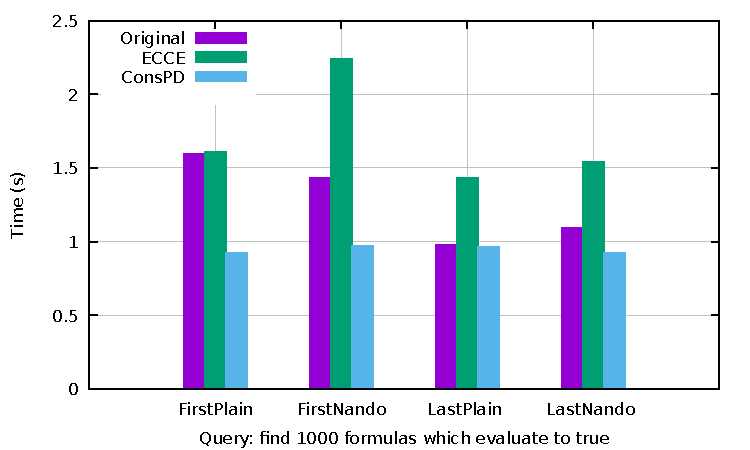
\includegraphics[width=0.65\textwidth]{pictures/prop/prop.pdf}
\end{center}
\end{frame}


\begin{frame}[fragile]
  \frametitle{Typechecker-Term Generator: Language}

\begin{figure}[!h]
  \resizebox{0.9\textwidth}{!}{
    \begin{minipage}{1.3\textwidth}
  \[\begin{array}{llll}
    term = &\ BConst \ of \ Bool &| \ IConst \ of \ Int &| \ Var \ of \ Int \\
    & | \ term + term &| \ term * term & \\
    & | \ term = term &| \ term < term & \\
    &| \ \underline{let} \ term \ \underline{in} \ term
    &\multicolumn{2}{l}{| \ \underline{if} \ term \ \underline{then} \ term \ \underline{else} \ term}
  \end{array}\]
  \caption{Language syntax}
    \end{minipage}
  }

\end{figure}




\begin{figure}[!h]
  \resizebox{0.9\textwidth}{!}{
    \begin{minipage}{1.3\textwidth}
  \setlength{\tabcolsep}{0.4cm}
  \begin{tabular}{c c c}
    \infer[]{\Gamma \vdash IConst \ i : Int}{} &
    \infer[]{\Gamma \vdash BConst \ b : Bool}{}  &
    \infer[\Gamma \lbrack v \rbrack \equiv \tau]{\Gamma \vdash Var \ v : \tau}{} \vspace{0.5cm}
    \\
    \infer[]{\Gamma \vdash t + s : Int}{\Gamma \vdash t : Int, \Gamma \vdash  s : Int}  \vspace{0.5cm} &
    \infer[]{\Gamma \vdash t = s : Bool}{\Gamma \vdash t : \tau, \Gamma \vdash  s : \tau} &
    \infer[]{\Gamma \vdash \underline{let} \ v \ b : \tau}{\Gamma \vdash v : \tau_v, \ (\tau_v :: \Gamma) \vdash b : \tau}
      \\

      \infer[]{\Gamma \vdash t * s : Int}{\Gamma \vdash t : Int, \Gamma \vdash  s : Int}  &
    \infer[]{\Gamma \vdash t < s : Bool}{\Gamma \vdash t : Int, \Gamma \vdash  s : Int} \vspace{0.5cm} &
      \infer[]{\Gamma \vdash \underline{if} \ c \ \underline{then} \ t \ \underline{else} \ s : \tau}{\Gamma \vdash c : Bool, \Gamma \vdash t : \tau, \Gamma \vdash s : \tau}
  \end{tabular}
  \vspace{-0.3cm}
  \caption{Typing rules implemented in typecheck$^o$ relation}
  \label{fig:typing}
\end{minipage}
  }
\end{figure}

\end{frame}

\begin{frame}[fragile]
  \frametitle{Typechecker-Term Generator: Evaluation}

Implementations:
\begin{itemize}
  \item Hand-coded typing rules in \mk
  \item Generated from functional typechecker by relational conversion
\end{itemize}

  \begin{center}
    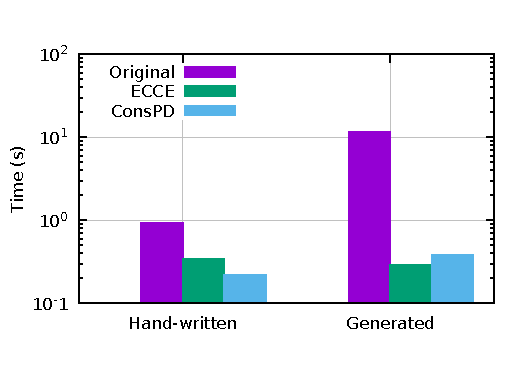
\includegraphics[width=0.65\textwidth]{pictures/type/ltypelog.pdf}
  \end{center}
\end{frame}

\begin{frame}[fragile]
  \frametitle{Discussion: Order of Answers}
Example from evalo.

Uselessness of measuring time.

Let's measure unifications
\end{frame}

\begin{frame}[fragile]
  \frametitle{Discussion: Deterministic Unfolding and Tupling}
maxlen works
maxmin does not work
\end{frame}


\begin{frame}[fragile]
  \frametitle{Conclusion}
  \begin{itemize}
    \item We developed and implemented Conservative Partial Deduction
    \begin{itemize}
      \item Less-branching heuristics
    \end{itemize}
    \item Evaluation shows some improvement, but not for every query
    \item Future work:
    \begin{itemize}
      \item Develop models to predict execution time
      \item Develop specialization which is more predictable, stable and well-behaved
    \end{itemize}
  \end{itemize}
\end{frame}


\end{document}
